\documentclass{article}
\usepackage[utf8]{inputenc}
\usepackage{graphicx}
\graphicspath{ {/images} }
\usepackage{lastpage}
\usepackage{titlesec}
\usepackage{parskip}
\usepackage{helvet}
\usepackage{soul}
\usepackage{statmath}
\renewcommand\familydefault{\sfdefault} 
\usepackage[T1]{fontenc}
\makeatletter
\usepackage[backend=biber,style=numeric-comp,sorting=none]{biblatex}
\addbibresource{Thesis.bib} %Import the bibliography file
\usepackage[table]{xcolor}
\usepackage{setspace}
\setstretch{1.15}
\DeclareBibliographyCategory{cited}
\AtEveryCitekey{\addtocategory{cited}{\thefield{entrykey}}}

\usepackage{geometry}
 \geometry{
 a4paper,
 right=24mm,
 top=24mm,
 left=24mm,
 bottom=24mm,
 }
\begin{document}

\begin{titlepage}

\begin{center}
\Large Methodology and Statistics for the Behavioural, Biomedical and Social Sciences\\
\vspace{0.15\textwidth}
\textbf{\LARGE PROPOSAL} 

\vspace{0.05\textwidth}

\rule{\textwidth}{1pt}\\[0.8cm]

\textbf { \LARGE Tuning strategies for hyperparameters of random forests}
\\ [0.5cm]

\rule{\textwidth}{1pt}

\vspace{0.1\textwidth}

\end{center}
\vspace{0.05\textwidth}
\begin{Large}
\begin{center}
    \textbf{Submitted by}\\ 
    Judith N\`eve --- 0070661\\
    \vspace{0.1\textwidth}
    \textbf{Supervisors}\\
    Dr. Maarten van Smeden\\
    Zo\"e Dunias\\

\vspace{0.15\textwidth}

\end{center}
\end{Large}

\vspace{0.2\textwidth}
\begin{large}
\textbf{Candidate journal}: \textit{Statistics in Medicine}\\
\textbf{FETC registration}: 22-1808\\
\textbf{Word count}: 749/750
\end{large}
\end{titlepage}

\newpage

\section{Introduction}

Machine learning models are increasingly used in medicine for diagnostic and prognostic purposes \cite{wessler_tufts_2017} assisting patients' medical decision-making. For this purpose, high \textit{classification accuracy} (i.e., the proportion of observations correctly classified) and \textit{discrimination} (i.e., the ability to differentiate between classes) are insufficient: models also need to be well \textit{calibrated} (i.e., risk predictions reflect patients' true risk) \cite{van_calster_calibration_2019}. Miscalibrated models can lead to over- or undertreatment if over- or underestimating patients' risks.\\

A popular set of techniques is tree-based methods \cite{mitchell_machine_1997}, among which random forests are particularly prevalent \cite{uddin_comparing_2019}. Random forests' results are influenced by hyperparameters (e.g. the minimum number of observations in a node) \cite{mantovani_empirical_2019}, which need to be set before fitting the model. While hyperparameter software defaults sometimes lead to appropriate discrimination \cite{bernard_influence_2009}, they can lead to severe miscalibration (work by Dunias, publication not yet available). It is then of utmost importance to identify hyperparameter tuning strategies improving calibration.\\

Tuning identifies hyperparameter values for which a metric (e.g. deviance) is optimal for a given model. Multiple elements need to be chosen before the tuning procedure can be carried out: the metric to optimise, the hyperparameters to tune, and the hyperparameter search algorithm. The latter two can greatly impact computation time: generally, the more hyperparameters are tuned, the larger computation time will be. Hyperparameter search algorithms may consider all possible values and combinations, or use information collected earlier in the tuning procedure to tune efficiently. Computation time is important to consider in conjunction to the improvement in model performance: greater computation times and longer training periods of models may lead to a strain on resources and increase carbon emissions. For complex models, this can be as much as five times the average emissions of a car over its lifetime \cite{strubell_energy_2019}.\\

Previous research suggests the most gain in random forest performance can be made by tuning the following hyperparameters: number of predictors sampled to make a split, proportion of the sample used to fit the tree, and minimum node size \cite{probst_tunability_2019}. Most hyperparameter search algorithms improve accuracy compared to default hyperparameters, with various effects on computational time (Figure 1) \cite{yang_hyperparameter_2020}.\\
\\
\centerline{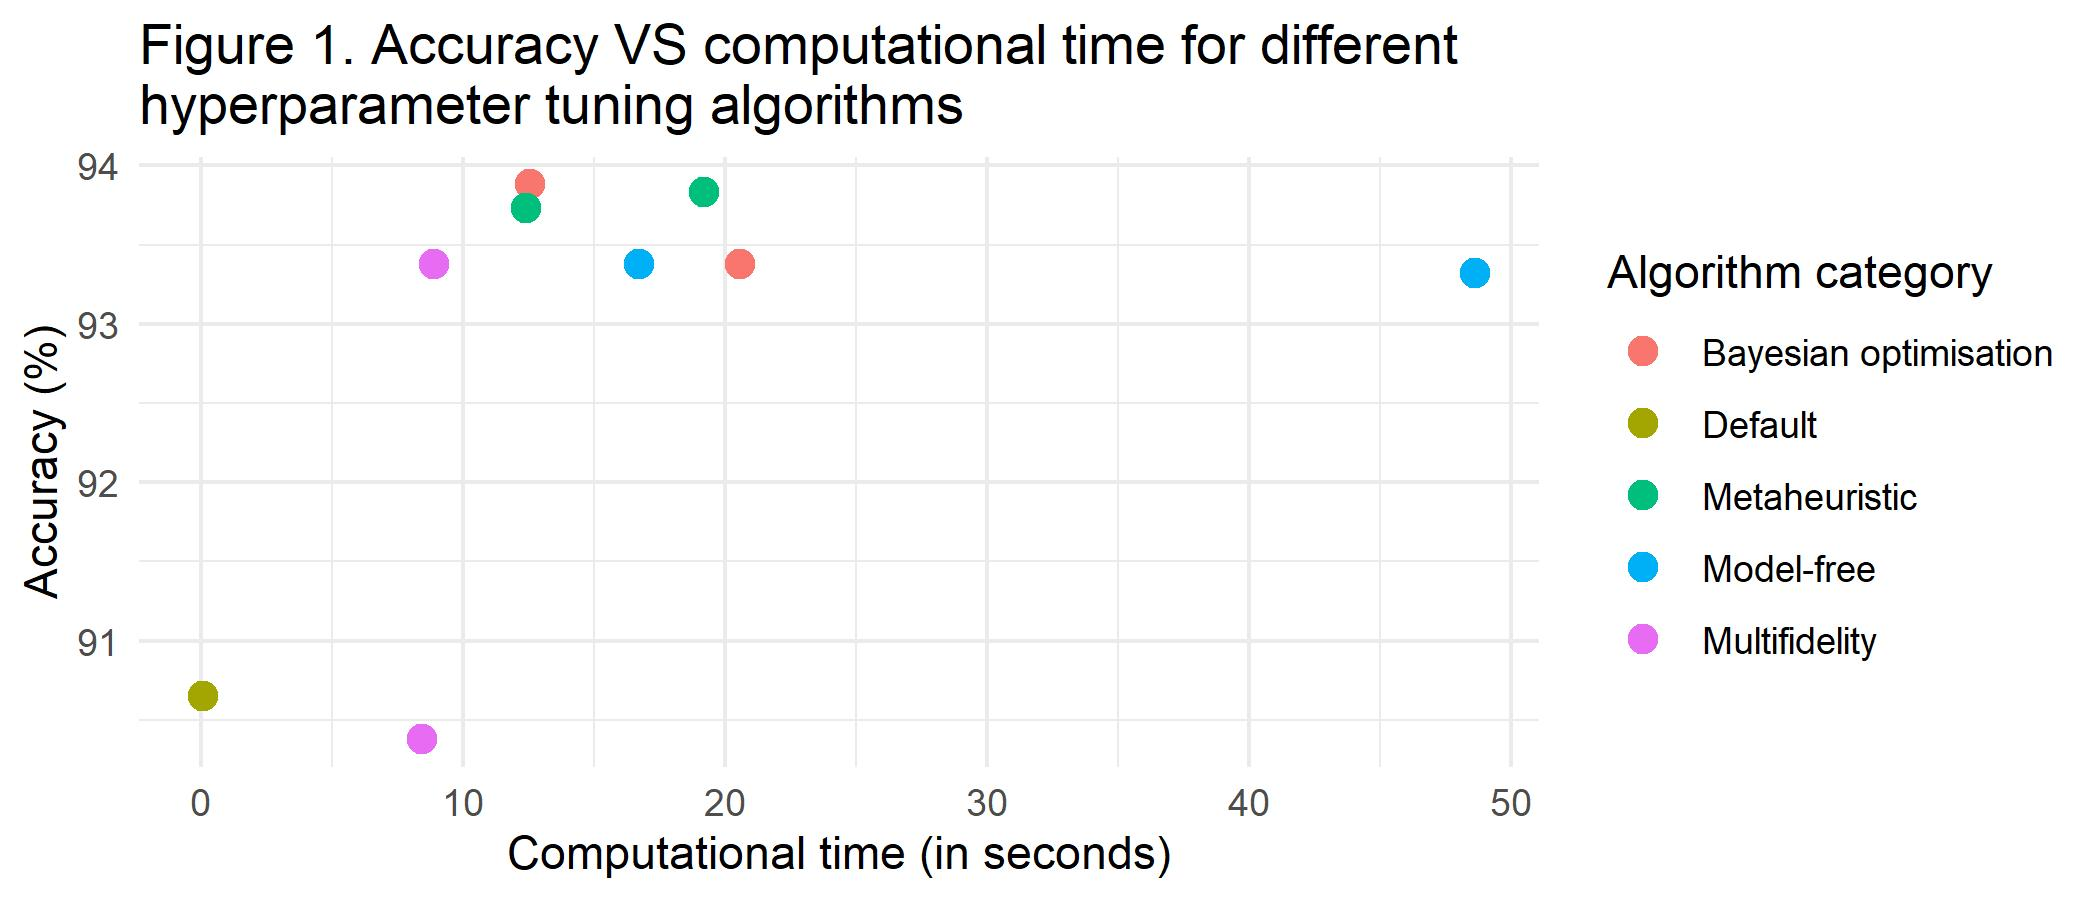
\includegraphics[height = 6cm]{figure1.jpg}}
\\
While there has been some focus on comparing hyperparameter search algorithms, so far, no study has compared different optimisation metrics' effects on model performance or computational time. Additionally, hyperparameter tuning has only been studied with accuracy as the outcome, not calibration or discrimination, which are typically more important in clinical settings.
\newpage
Larger computational time does not necessarily lead to an improvement in accuracy. It is unknown whether there is a point at which continuing a search algorithm no longer leads to improvements in model calibration and discrimination. The current project will thus address the following question: what are the optimal hyperparameter tuning strategies for balancing predictive performance and computational time of tree-based methods in low-dimensional settings?

\section{Analytical strategy}

There will be three simulation studies in this project to identify which hyperparameters to tune, which metric to optimise, and which search algorithm to use for optimal model performance. All studies will follow the ADEMP \cite{morris_using_2019} approach to simulation studies. All studies will be conducted using 1000 simulated datasets per scenario, of which the following characteristics will vary: number of candidate predictors (8, 16, 32), event fraction (i.e., the proportion of individuals with the predicted outcome; 0.1, 0.3, 0.5), and sample size (required sample size calculated using \cite{riley_calculating_2020}, half the required sample size, twice the required sample size).\\

Study 1 will aim to identify hyperparameters with the most impact on model performance. We expect similar results to those of Probst and colleagues \cite{probst_tunability_2019}. Study 2 will aim to identify an optimisation metric leading to better calibration performance. We expect all metrics to perform similarly. Study 3 will aim to identify the best hyperparameter search algorithm for model performance and computational time. We aim to identify a more efficient and better performing search algorithm than the standardly used grid search, extending prior findings \cite{yang_hyperparameter_2020} on model predictive performance.\\

Settings for the three simulation studies are summarised in Table 1. All analyses will be conducted in R on a high-performance computer, with the exception of search algorithms in study 3. These will be run in Python.\\

Table 1: settings for each simulation study\\
\rowcolors{2}{gray!10}{gray!40}
\begin{tabular}{>{\raggedright\arraybackslash}p{4cm}>{\raggedright\arraybackslash}p{2.5cm}>{\raggedright\arraybackslash}p{2.5cm}>{\raggedright\arraybackslash}p{3cm}>{\raggedright\arraybackslash}p{3cm}}
    \hline
    Study &
    Metric &
    Hyperparameters to tune &
    Search algorithm &
    Outcome measure\\
    \hline
    \textbf{Study 1} &
    Deviance &
    All hyperparameters &
    Grid search &
    Calibration slope \newline AUC\\
    \textbf{Study 2} &
    Deviance \newline Brier score \newline Accuracy \newline Logarithmic loss &
    Selected from study 1 &
    Grid search &
    Calibration slope \newline AUC\\
    \textbf{Study 3} &
    Selected from study 2 &
    Selected from study 1 &
    Grid search \newline Random search \newline Gradient-based optimisation \newline BO-TPE \newline Hyperband \newline GA &
    Calibration slope \newline AUC \newline Computation time\\
    \hline
\end{tabular}
\\

Using results from each of the simulations, we will conclude the study with a recommendation regarding which metric to optimise, which hyperparameters to tune, and which search algorithm to use for common situation in medical prediction modeling. Information will however be available regarding the cost of other approaches such that future research will be able to make an informed decision best suited for the purpose of the studies.

\newpage

\nocite{*}
\printbibliography[title={References},category=cited]
\printbibliography[title={Further Reading},notcategory=cited]

%\textbf{Reference list\\
%-	Add a reference list for the literature used in the text – you can use the formatting style of the chosen journal, but this is not mandatory.\\
%-	Add about 20 extra references that will be used for the thesis (you do not have to have read these already).}

\end{document}
